
%--------------------------------------------------------------
% ĐẠI HỌC BÁCH KHOA HÀ NỘI
% Trường Điện - Điện tử
% Khoa Tự động hoá
%
% MẪU SOẠN THẢO ĐỒ ÁN

% Phiên bản bổ sung ghi chú sửa đổi, kế hoạch thực hiện và biên bản cuộc họp theo mẫu của thầy Nguyễn Quốc Cường - Smart Sensor Lab
%--------------------------------------------------------------

\documentclass{thesis}
\usepackage[utf8]{inputenc} % 
\usepackage[T5]{fontenc} % Font Vietnamese
\usepackage{graphicx} % Figure
\usepackage{float} % Set position figure or table
\usepackage{mathptmx} % select font Times New Roman
\usepackage{geometry} % Set parameters paper
\usepackage{xcolor}
\usepackage[fontsize=13pt]{scrextend} % set font size = 13pt
% \usepackage{indentfirst} % Indent first line
\usepackage[protrusion=false]{microtype}
\usepackage{titling}
\usepackage{multicol}

\usepackage{amsmath} % for math equation

\usepackage{siunitx} % for unit
\usepackage{longtable} % for long table
% \usepackage{subfigure}
\usepackage{subcaption}
\usepackage{enumitem}

% Set global spacing for itemize
\setlist[itemize]{itemsep=2pt, topsep=3pt, left=1cm}
\linespread{1.15}

\nocite{*}


%% START DOCUMENT
\begin{document}

% CREATE COVER PAGE
% CREATE COVER PAGE

\begin{center}
    \vspace{12pt} % line spacing
        \textbf{\fontsize{15pt}{0pt} \selectfont{} ĐẠI HỌC BÁCH KHOA HÀ NỘI }
    \vspace{0.5cm}
    
% INSERT LOGO
\begin{figure}[H]
    \centering
    
\includegraphics[width=2cm,height=3cm]{logoBK.png}
\end{figure}

% THESIS TYPE
\vspace{48pt}
        \fontsize{25pt}{0pt}{\fontfamily{qag}\selectfont{} \textbf{ĐỒ ÁN TỐT NGHIỆP}
}
\vspace{24pt}

 % THESIS TITTLE
        \fontsize{17pt}{0pt}{\fontfamily{qag}\selectfont{} \textbf{   
        THIẾT KẾ THIẾT BỊ ĐỌC GHI
        MÀN HÌNH CỘT BƠM \\ XĂNG DẦU
        }}
\vspace{18pt}

% NAME
        \fontsize{14pt}{0pt}\selectfont{} \textbf{NGUYỄN THÁI SƠN}
    \vspace{3pt}

% EMAIL    
        \fontsize{14pt}{0pt}\selectfont{} son.nt212951@sis.hust.edu.vn
    \vspace{12pt} % line spacing

% MAJOR
        \fontsize{14pt}{0pt}\selectfont{} \textbf{Ngành Kỹ thuật Điều khiển và Tự động hóa}  
\end{center}
    \vspace{48pt}

% INFORMATION: SUPERVISOR NAME, STUDENT NAME,...
\begin{table}[H]
    \centering
        \begin{tabular}{l l c}
            \textbf{Giảng viên hướng dẫn:}    &  PGS.TS. Nguyễn Quốc Cường \vspace{6pt} & \\
            &\vspace{3pt} & \fontsize{10pt}{0pt}\selectfont{} Chữ ký của GVHD \\
            \textbf{Khoa:} & Tự động hóa \vspace{3pt}\\ 
            \textbf{Trường:} & Điện - Điện tử
        \end{tabular}
\end{table}

% TIME
\begin{center}
    \vspace{48pt}
    \fontsize{14pt}{0pt}\selectfont{} \textbf{Hà Nội, 3/2025}
\end{center}
    \newpage
   %     \clearpage
%            \thispagestyle{empty}
  %              \cleardoublepage

% THESIS TASK                
% THESIS TASK                
\begin{multicols}{2}
\centering
\hspace{-3cm}BỘ GIÁO DỤC \& ĐÀO TẠO \\ \hspace{-3cm}\textbf{ĐH BÁCH KHOA HÀ NỘI}

\columnbreak

\hspace{-1.6cm}\textbf{CỘNG~HÒA~XÃ~HỘI~CHỦ~NGHĨA~VIỆT~NAM} \\ \hspace{-1.6cm}\textbf{Độc lập -- Tự do -- Hạnh phúc}

\end{multicols}

\begin{center}
   \textbf{NHIỆM VỤ \\ĐỒ ÁN TỐT NGHIỆP} 
\end{center}

%\raggedright

\hspace{-1cm}Họ và tên sinh viên: Nguyễn Thái Sơn\\Khóa: K66 \hfill Trường: Điện -- Điện tử \hfill Ngành: KT ĐK \& TĐH
    
    % Thay các dấu chấm (\ldots) dưới đây bằng nội dung
    
    \hspace{-1cm}\textit{1. Tên đề tài}\\
             Thiết kế thiết bị đọc ghi màn hình cột bơm xăng dầu  \\[0.2cm]
    \textit{2. Nội dung đề tài}\\
            Thiết kế và triển khai hệ thống gồm phần cứng và phần mềm
            để thu dữ liệu hiển thị trên màn hình cây xăng, giải mã
            và lưu các lượt bơm xăng. Lấy mẫu thông tin màn hình với tần số 100Hz. Có kết nối mạng LAN với máy tính nội bộ. Thiết bị có giao diện giám sát và điều khiển dạng Web App.

            Các công việc bao gồm:
            \begin{itemize}
                \item Thiết kế mạch thu dữ liệu màn hình
                \item Thu thập và phân tích tín hiệu gửi tới màn hình
                \item Thiết kế bộ giải mã dữ liệu
                \item Triển khai hệ thống mạng và phần mềm để thu và giải mã dữ liệu màn hình theo thời gian thực
                \item Triển khai cơ sở dữ liệu và giao diện hiển thị dữ liệu màn hình
                \item Chạy kiểm thử hệ thống tại hiện trường
            \end{itemize}
           
    \textit{3. Thời gian giao đề tài: 18/02/2025} \\[0.2cm]

    \textit{4. Thời gian hoàn thành: dd/mm/yyyy} \\[0.2cm]

\vspace{6pt}
\hspace{7cm}\textit{Ngày (dd) tháng (mm) năm 202y}\\
\vspace{2pt}
\hspace{8.5cm}\textbf{CÁN BỘ HƯỚNG DẪN} \\

\vspace{36pt}

\hspace{8cm}\textbf{Nguyễn Quốc Cường}
    \newpage
%        \clearpage
 %           \thispagestyle{empty}
 %               \cleardoublepage    
                
% THANKS
% THANKS
\section*{LỜI CẢM ƠN}
    \thispagestyle{empty}
Đây là mục tùy chọn, nên viết phần cảm ơn ngắn gọn, tránh dùng các từ sáo rỗng.

\vspace{6pt}
    \hspace{7cm}Hà Nội, ngày 24 tháng 03 năm 2025
        
        \hspace{8.6cm} Sinh viên thực hiện      % command '\hspace' used to line indents

\vspace{2cm}
    \hspace{8.8cm}\textbf{Nguyễn Thái Sơn} % change name

\newpage % create a new page
%    \thispagestyle{empty} 
%        \clearpage
%            \thispagestyle{empty}
  %              \cleardoublepage

% SUMMARY PART
% SUMMARY PART
\section*{TÓM TẮT ĐỒ ÁN}
    \thispagestyle{empty}
(Sẽ được bổ sung vào giai đoạn cuối của đồ án)


\newpage

% TABLE OF CONTENT
\tableofcontents 
    \thispagestyle{empty}
        \newpage
 %           \thispagestyle{empty}
  %              \cleardoublepage

% LIST OF SYMBOLS AND ABBREVIATIONS
\pagenumbering{roman}   % Roman numbering: i, ii, iii, iv,...
\section*{DANH MỤC KÝ HIỆU VÀ CHỮ VIẾT TẮT}
    \phantomsection \addcontentsline{toc}{section}{\numberline{} DANH MỤC KÝ HIỆU VÀ CHỮ VIẾT TẮT}

% Create table
\begin{tabular}{ l l }
    \hspace{1cm} HESS & \hspace{4cm} Hybrid Energy Storage System \\  
    \hspace{1cm} SC & \hspace{4cm} Super Capacitor    \\
    \hspace{1cm} EMS  & \hspace{4cm} Energy Management Strategy 
\end{tabular}  
    \newpage

% LIST OF FIGURES
{\let\oldnumberline\numberline
    \renewcommand{\numberline}{Hình~\oldnumberline}
        \listoffigures}
            \phantomsection\addcontentsline{toc}{section}{\numberline{} DANH MỤC HÌNH VẼ}
\newpage

% LIST OF TABLES
{\let\oldnumberline\numberline
    \renewcommand{\numberline}{Bảng~\oldnumberline}
        \listoftables}
            \phantomsection\addcontentsline{toc}{section}{\numberline{} DANH MỤC BẢNG BIỂU}
\newpage

%%%%%%%%%%%% Using for lab report version %%%%%%%%%%%%
\section*{Bảng cập nhật báo cáo} \label{edit_note}

\begin{center}
    \begin{longtable}{|>{\centering\arraybackslash}p{1cm}|>{\raggedright\arraybackslash}p{4cm}| >{\raggedright\arraybackslash}p{10cm}|}
    \caption{Bảng cập nhật báo cáo.}
    \\
        \hline
        \textbf{Ngày} & \textbf{Nội dung báo cáo} & \textbf{Sửa đổi / ghi chú} \\
        \hline
        \endhead
      
        4/3 & Bảng kế hoạch & Lập bảng kế hoạch công việc \\

        24/3 & Chương 1: Tổng quan hệ thống & Viết nội dung tổng quan hệ thống \\

        25/3 & Meeting note & Ghi các meeting note vào báo cáo \\

        \hline
    \end{longtable}
\end{center}
\thispagestyle{empty}
\newpage

\section*{Kế hoạch thực hiện} \label{Implementation_plan}

\begin{longtable}{|>{\centering\arraybackslash}p{1cm}| >{\raggedright\arraybackslash}p{3cm}| >{\raggedright\arraybackslash}p{7cm}| > {\raggedright\arraybackslash}p{3cm}|}
    \caption{Bảng kế hoạch dự án.}
    \label{tab:plan_project}
    \\
        \hline
        Tuần & Nhiệm vụ & Yêu cầu cần đạt & Trạng thái \\
        \endhead
        
        \hline
        26 & Xác định mục tiêu đề tài & Liệt kê yêu cầu bài toán, chức năng thiết bị & Hoàn thành \\
        
        \hline
        27 & Tìm hiểu đặc điểm cột bơm, xác định phạm vi bài toán & Báo cáo trình bày đặc điểm cột bơm & Hoàn thành \\

        \hline
        28 & Lập bảng kế hoạch công việc & File Excel có bảng liệt kê các đầu việc chi tiết cho các tuần cùng với tiến độ được cập nhật &  Hoàn thành \\
        
        \hline
        29 & Vẽ sơ đồ hệ thống & Sơ đồ tổng quan hệ thống & Hoàn thành \\

        \hline
        30 & Liệt kê và tìm hiểu các công nghệ sử dụng & Báo cáo tìm hiểu các phần tử IC được sử dụng, CPLD và STM32 & Hoàn thành \\

        \hline 
        31 & Tìm hiểu mạch cứng & Đọc hiểu và viết tài liệu về mạch cứng, tìm hiểu các linh kiện & Đang thực hiện \\

        \hline
        32 & Vẽ thiết kế mạch cứng & Bản thiết kế mạch cứng & Chưa làm \\
        
        \hline 
        32 & Triển khai hệ thống phần mềm & Xây dựng kiến trúc source code và chuẩn API & Chưa làm \\

        \hline
        33 & Triển khai  backend server & Demo backend server giao tiếp bằng chuẩn API đã đưa ra & Chưa làm \\

        \hline 
        34 & Triển khai giao diện hiển thị & Demo giao diện mô phỏng màn hình cây xăng theo thời gian thực & Chưa làm\\

        \hline 
        35 & Kiểm thử, chạy thử hệ thống và quay video demo & Demo chạy thử toàn hệ thống, trình bày các lỗi phát sinh nếu có & Chưa làm \\
        
        \hline 
        36 & Viết báo cáo quyển & Trình bày quyển & Chưa làm \\

        \hline 
        37 & Viết báo cáo dạng báo cáo khoa học & Trình bày báo cáo & Chưa làm \\

        \hline

\end{longtable}
\thispagestyle{empty}
\newpage

\section*{Biên bản cuộc họp} \label{tab:Meeting_notes}

\begin{longtable}{|>{\centering\arraybackslash}p{1cm}| >{\raggedright\arraybackslash}p{4cm}| >{\raggedright\arraybackslash}p{5cm}| > {\raggedright\arraybackslash}p{4cm}|}
    \caption{Biên bản cuộc họp.}
        \\
        \hline
        Ngày & Nội dung & Quyết định & Nhiệm vụ tiếp theo \\
        \endhead
       
        \hline
        25/2 & Giao đề tài và nêu ý tưởng chung về đề tài & Đưa ra các đầu việc, thống nhất về đầu mối & Tìm hiểu công nghệ, dựng hệ thống và tài liệu hóa  \\

        \hline
        4/3 & Trình bày sơ bộ về tiến độ, bảng kế hoạch (đã đưa và đang chờ duyệt). Thống nhất lịch họp hàng tuần & Khoảng hết tuần 5, đầu tuần 6 báo cáo overview và kế hoạch đồ án & Bắt đầu viết tài liệu hệ thống \\

        \hline
\end{longtable}
\thispagestyle{empty}
\newpage

%%%%%%%%%%%%%%%%%%%%%%%%%%%%%%%%%%%%%%%%%%%%%%%%%%%%%%%%%%%%

%% --------------------------------------------------%%
%------------CHAPTER 1---------------------------%
%%-----------------------------------------------------%

\pagenumbering{arabic} % numbering: 1,2,3,...
    \section*{CHƯƠNG 1. GIỚI THIỆU CHUNG} 
        \addcontentsline{toc}{section}{\numberline{}CHƯƠNG 1. GIỚI THIỆU CHUNG} % Reference to content

\setcounter{section}{1} 
    \setcounter{subsection}{0}
        \setcounter{figure}{0}
            \setcounter{table}{0}
%%--------------------------------------------------------

\subsection{Vai trò của thiết bị đọc ghi màn hình cột bơm xăng dầu}

\hspace{1cm} Công nghệ số mang đến ngày càng nhiều lợi ích to lớn về mặt tiện dụng, hiệu quả và tiết kiệm thời gian cho doanh nghiệp cũng như người dùng. Từ đó, nhu cầu lớn về chuyển đổi số được phát sinh. Các thông tin giao dịch, hóa đơn trên giấy tờ ngày càng được thay thế bằng các giao dịch, hóa đơn điện tử, thuận tiện cho truyền tải thông tin, lưu trữ và quản lý. Các hệ thống trạm xăng và cột bơm cũng không phải ngoại lệ với nhu cầu đó, các giao dịch, lượt bơm xăng cũng cần được ghi lại dưới dạng dữ liệu số để gửi lên máy chủ của doanh nghiệp, thuận tiện lưu trữ và thống kê một cách chính xác, ổn định và giảm hoặc triệt tiêu những lỗi con người có thể gây ra.

Những cột bơm mới được bán gần đây cũng đã được sản xuất tích hợp chức năng xuất hóa đơn điện tử. Nhưng còn một lượng rất lớn những cây xăng với công nghệ cũ vẫn còn đạt tiêu chuẩn và sử dụng tốt được ở nhiều trạm bơm trên khắp cả nước, việc bỏ hẳn những cây xăng này đi thay bằng những cây xăng công nghệ mới sẽ tốn nhiều thời gian và chi phí đầu tư, gây lãng phí cũng như thải nhiều rác thải điện tử hơn cho môi trường. Từ đó xuất hiện nhu cầu cải tiến những cây xăng cũ để xuất được hóa đơn điện tử, chi phí và thời gian doanh nghiệp bỏ ra sẽ được tối ưu hơn.

Từ yêu cầu trực tiếp của doanh nghiệp, báo cáo này được viết để đưa ra phương án thiết kế và triển khai hệ thống có thể đọc ghi và giải mã, phân tích dữ liệu màn hình cây xăng, từ đó phát hiện được các lần giao dịch và lưu trữ, quản lý các lượt giao dịch - lượt bơm xăng đó.


\subsection{Khái quát về yêu cầu và chức năng của hệ thống}



\begin{figure}[!ht]
    \centering
    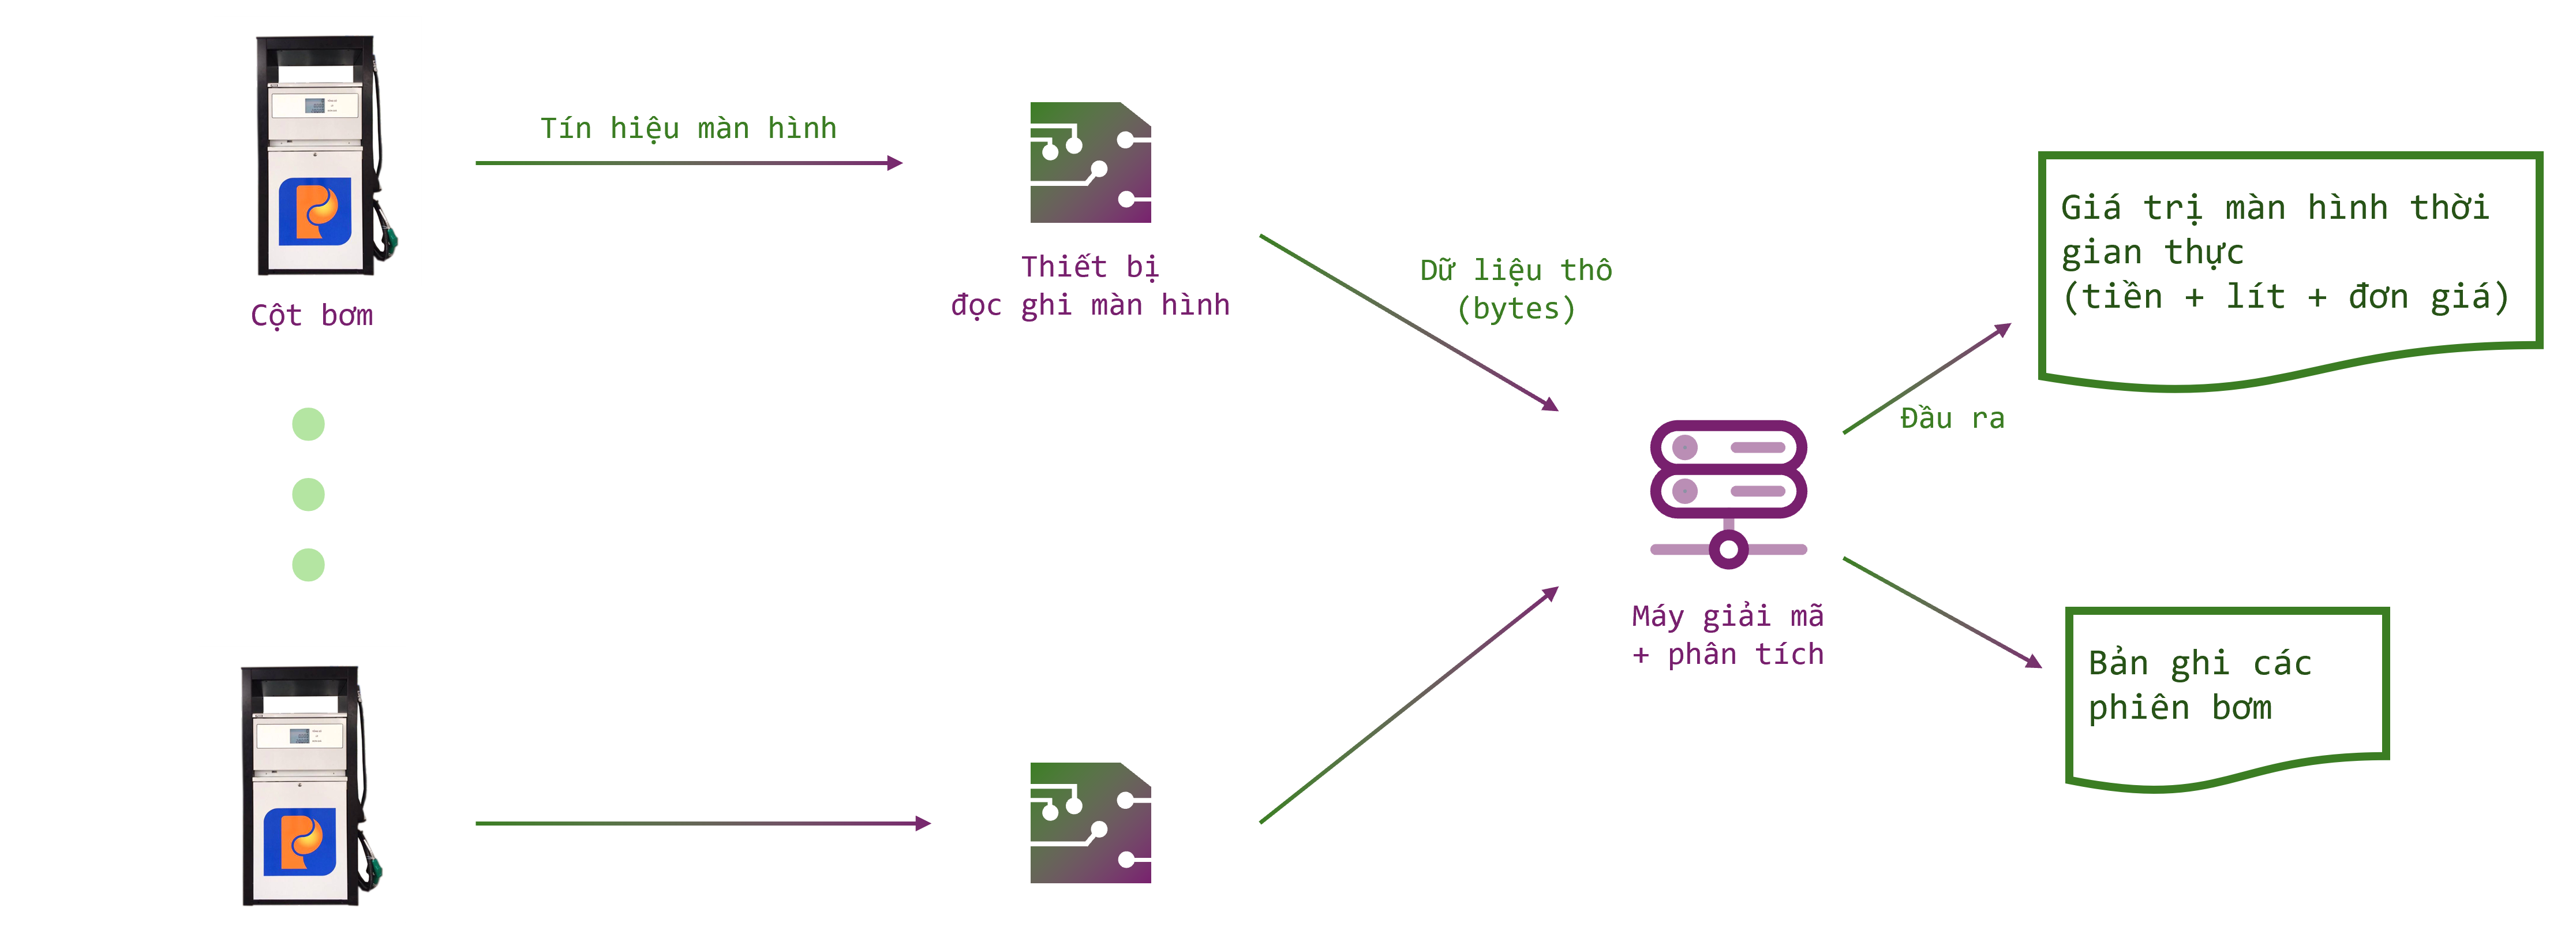
\includegraphics[width=1.0\linewidth]{Figures/Chap1_proj-purpose.png}
    \caption{Minh họa mục tiêu đầu ra của hệ thống}
    \label{fig:hinh1.1}
\end{figure}

Mục tiêu là thiết kế thiết bị đọc ghi và giải mã màn hình cây xăng đáp ứng những nhu cầu sau:

 \textbf{1. \quad Giám sát số liệu hiển thị trên cột bơm theo thời gian thực}

 Hệ thống có thể đọc và hiển thị trực tiếp dữ liệu cột bơm theo thời gian thực bao gồm: số tiền, số lít và đơn giá. Người dùng có thể theo dõi trạng thái hiển thị của cột bơm ngay tại phòng điều khiển mà không cần quan sát trực tiếp màn hình cột.
 

 \textbf{
    2. \quad  Phát hiện các lượt bơm hoàn chỉnh
 }

 Thông qua các số liệu thời gian thực (số tiền, số lít, đơn giá) của cột bơm, hệ thống phát hiện được đâu là bắt đầu và kết thúc của một lượt bơm xăng, thông báo một lượt bơm/hóa đơn hoàn chỉnh.


 \textbf{
    3. \quad Lưu trữ và hiển thị các lượt bơm
 }

 Các lượt bơm được lưu trữ trong cơ sở dữ liệu, tạo cơ sở để có thể xuất các hóa đơn điện tử.


 \textbf{
    4. \quad Hỗ trợ điều khiển từ xa
 }

 Việc ghi dữ liệu cột bơm có thể được điều khiển bật tắt từ xa, thông qua giao diện phần mềm.


 \textbf{
    5. \quad Cập nhật phần mềm từ xa (OTA)
 }

 Hỗ trợ cập nhật phần mềm từ xa, cho phép người dùng cập nhật phiên bản mới từ giao diện người dùng để có tối ưu những tính năng, tiện ích mới nhất từ phiên bản phần cứng đã có.

Thông qua việc triển khai mục tiêu trên, đề tài hướng tới tạo ra một hệ thống đọc và giải mã màn hình cây xăng hoàn chỉnh, đáp ứng nhu cầu quan sát từ xa các cột bơm theo thời gian thực, tự động phát hiện và ghi lại được các lượt bơm, tạo tiền đề để phát triển các ứng dụng như là xuất hóa đơn điện tử, thanh toán không chạm, và các ứng dụng khác.

\subsection{Phạm vi nghiên cứu}

\hspace{1cm} Thiết bị đọc ghi màn hình cột bơm xăng dầu có thể đọc ghi và giải mã loại cột bơm truyền thống có đặc điểm sau:
\begin{itemize}
   \item Hãng sản xuất: ZCheng
   \item Loại cáp màn hình: 8P 3.96mm
   \item Số lượng chân cáp: 8
   \item Số chân tín hiệu của cáp: 3
   \item Giao thức: SPI
   \item Độ lớn frame: 22 byte
   \item Bit rate: 400Kb/s
   \item Tần số frame: 100Hz
\end{itemize}
Đây là loại cột bơm cũ phổ biến tại các trạm xăng trên thị trường. Phạm vi chức năng của hệ thống bao gồm:

 \textbf{1. \quad Giám sát số liệu hiển thị trên cột bơm theo thời gian thực}

 Thu và giải mã dữ liệu SPI gửi tới màn hình thiết bị. Hiển thị giá trị màn hình (số tiền, số lít, đơn giá) theo thời gian thực trên giao diện người dùng.

  \textbf{
    2. \quad  Phát hiện các phiên bơm hoàn chỉnh
 }

 Sau khi bơm xăng, người vận hành dừng bơm một thời gian (5s) hoặc nhấn nút reset để bắt đầu phiên bơm mới, thiết bị phát hiện và ghi lại giá trị màn hình hiện tại thành một phiên bơm.

  \textbf{
    3. \quad Lưu trữ và hiển thị các lượt bơm
 }

 Các bản ghi phiên bơm được lưu vào cơ sở dữ liệu ngay trên máy tính nội bộ và hiển thị lên giao diện quản lý

 \textbf{
    4. \quad Hỗ trợ điều khiển từ xa
 }

Thiết bị đọc màn hình cây xăng có 2 relay đóng ngắt có thể nối nối tiếp vào cột bơm. Từ giao diện quản lý, có thể điều khiển relay đóng ngắt bằng nút ấn trên giao diện.


 \textbf{
    5. \quad Cập nhật phần mềm từ xa (OTA)
 }

 Từ giao diện quản lí, có thể tải (upload) file phần mềm dạng mã nhị phân, gửi cho thiết bị đọc màn hình để thiết bị tự cập nhật. 

\subsection{Phương pháp nghiên cứu}

\hspace{1cm} Bối cảnh màn hình cây xăng là các màn hình cũ, không có tài liệu cụ thể về thiết phần cứng và giao thức.

\begin{figure}[!ht]
    \centering
    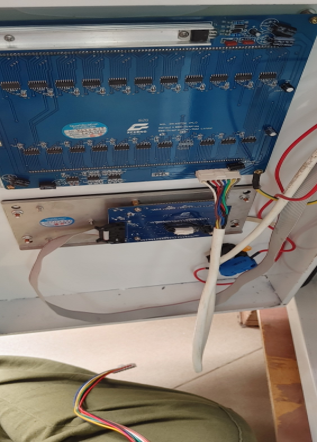
\includegraphics[width=0.5\linewidth]{Figures/Chap1_Zcheng-screen-hardware.png}
    \caption{Mạch phần cứng màn hình cây xăng hãng ZCheng}
    \label{fig:hinh1.1}
\end{figure}

Do đó, cần khảo sát tín hiệu màn hình. Sử dụng mạch thu và phần mềm của Logic Analyzer để thu tín hiệu theo các bước sau:

- Sử dụng đồng hồ đo áp, xác định các chân nguồn, đất, tín hiệu và các chân có điện áp cao (để tránh cắm chân Logic Analyzer vào các chân có điện áp cao này).

- Sử dụng mạch cứng và phần mềm Logic Analyzer nối vào các chân tín hiệu tới màn hình để thu các tín hiệu. Đồng thời, sử dụng máy quay quay lại màn hình hiển thị trong quá trình thu.

- Thực hiện các thao tác phổ biến: reset màn hình, bơm xăng, preset màn hình (đặt trước giá trị tiền hoặc lít cần bơm) rồi ghi lại tín hiệu và video màn hình trong quá trình vận hành thao tác.

- Khảo sát tín hiệu, so sánh tín hiệu với giá trị hiển thị trên màn hình để xác định:

\begin{itemize}
   \item Vị trí các chân (nguồn, đất, cấp xung, dữ liệu, ...)
   \item Giao thức sử dụng (SPI), dấu hiệu bắt đầu và kết thúc một gói tin
   \item Ý nghĩa các byte trong gói tin
\end{itemize}

Từ đó, chế tạo mạch thu gói tin theo giao thức SPI và thiết kế phần mềm giải mã.

\subsection{Cấu trúc đồ án}

Nội dung được trình bày ở các chương tiếp theo bao gồm: 
\begin{itemize}
   \item Tổng quan lý thuyết và công nghệ: Trình bày các nền tảng lý thuyết và mô tả các công nghệ được sử dụng trong thiết kế.
   \item Thiết kế hệ thống sản phẩm: Bao gồm sơ đồ các khối chức năng của thiết bị đọc ghi màn hình và phần mềm giải mã, cùng với thiết kế chi tiết (mạch cứng và phần mềm) từng khối, trình tự giao tiếp giữa các khối.
   \item Triển khai và thử nghiệm: Thử nghiệm thiết bị trên màn hình cột bơm tại hiện trường, đánh giá kết quả.
   \item Kết luận và hướng phát triển.
\end{itemize}

\subsection{Kết luận chương}

\hspace{1cm} Trong chương này, em đã đưa ra bối cảnh thực tế của bài toán, giải thích nhu cầu thực tế của thiết bị đọc ghi màn hình cây xăng, cùng với lợi ích mà nó mang lại trong quá trình phát triển và chuyển đổi số.

Đồng thời, chương này liệt kê các yêu cầu kĩ thuật cụ thể, cách tiếp cận bài toán từ đó đưa ra hướng thiết kế và triển khai tiếp theo.



\newpage
%---------------------------------------------------------%%
%% ----------CHAPTER 2 -------------------%%
%---------------------------------------------------------%%

\section*{CHƯƠNG 2. CƠ SỞ LÝ THUYẾT}
    \addcontentsline{toc}{section}{\numberline{} CHƯƠNG 2. CƠ SỞ LÝ THUYẾT}

\setcounter{section}{2}
    \setcounter{subsection}{0}
        \setcounter{figure}{0}
            \setcounter{table}{0}
%---------------------------------------------------------%

\subsection{}

\newpage

%% --------------------------------------------------%%
%------------CHAPTER 3---------------------------%
%%-----------------------------------------------------%

\section*{CHƯƠNG 3. THIẾT KẾ HỆ THỐNG}
    \addcontentsline{toc}{section}{\numberline{}CHƯƠNG 3. PHƯƠNG PHÁP LUẬN}
    
\setcounter{section}{3}
    \setcounter{subsection}{0}
        \setcounter{figure}{0}
            \setcounter{table}{0}
%%-------------------------------------------------------%%
% --------------------------------------------------------%
%---------------------------------------------------------%

\subsection{Phân tích yêu cầu hệ thống}


\begin{figure}[!ht]
    \centering
    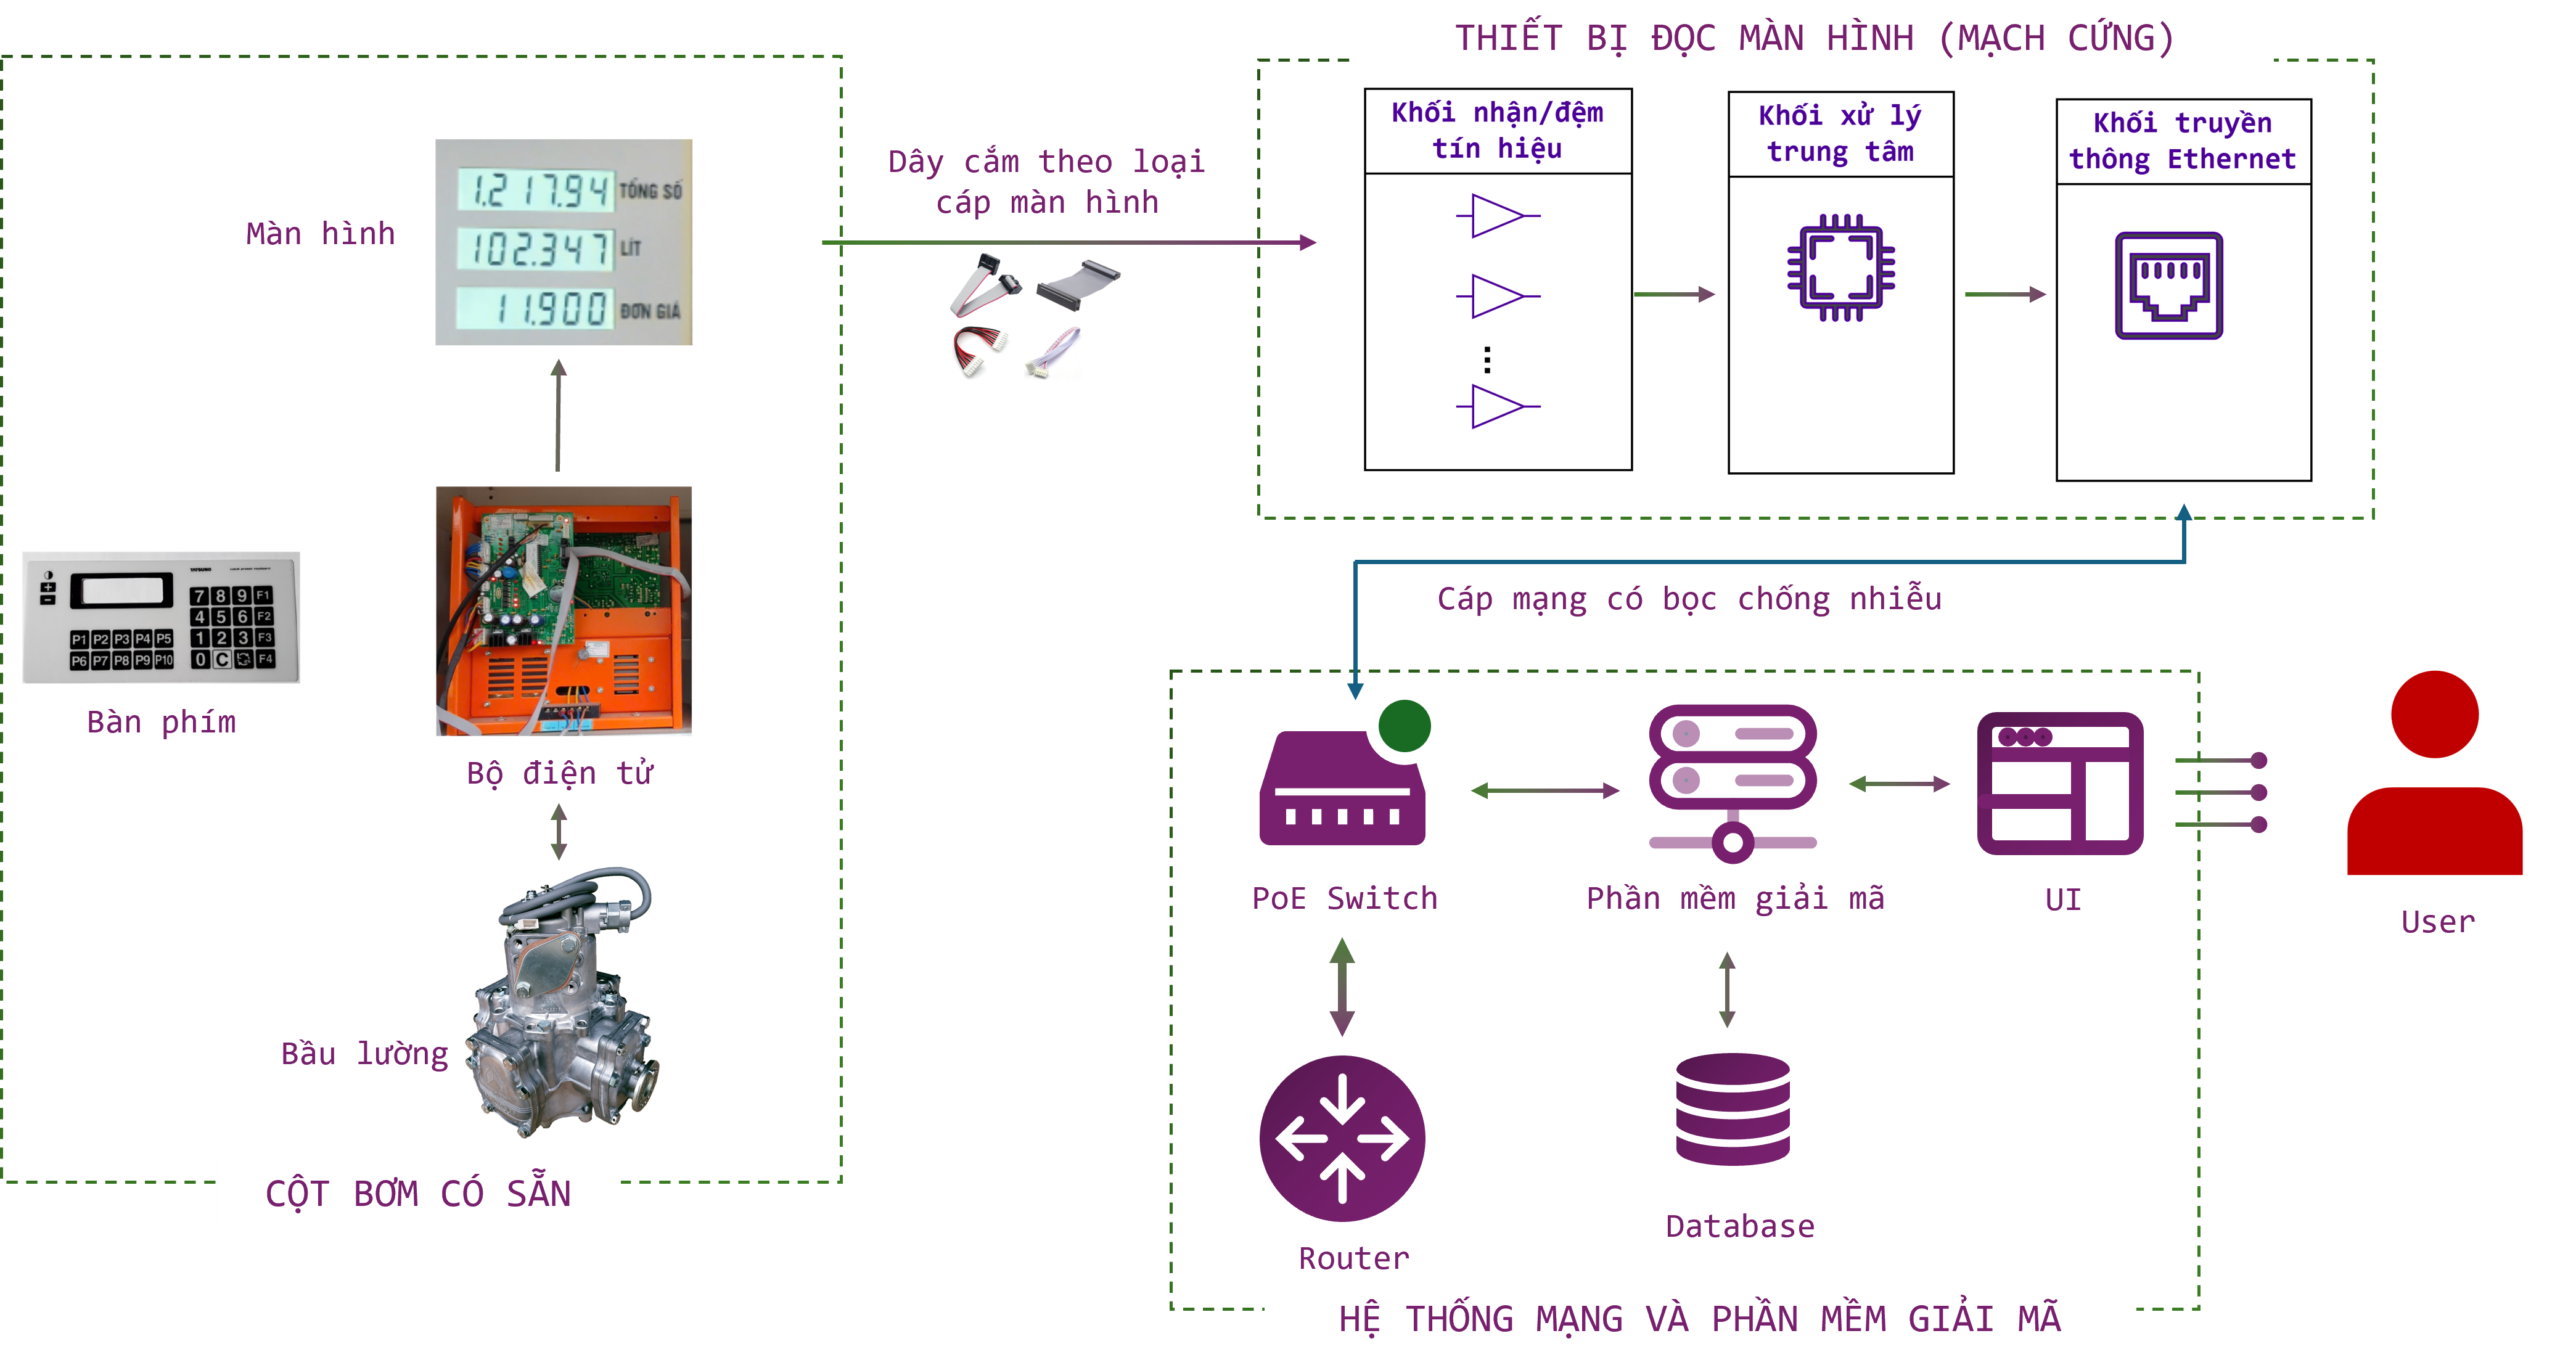
\includegraphics[width=1.0\linewidth]{Figures/Chap3_FunctionBlock-implementation.png}
    \caption{Các thành phần của hệ thống}
    \label{fig:hinh3.1}
\end{figure}

Các thành phần chính của hệ thống bao gồm:

\subsubsection{Thiết bị đọc ghi màn hình}


\hspace{0.8cm} Là mạch cứng gắn vào màn hình cột bơm, thu dữ liệu thô màn hình:
\begin{itemize}
   
    \item Kích cỡ: vừa, có thể lắp đặt trong cột bơm
    \item Tần số lấy mẫu: 100Hz
    \item Cấp nguồn riêng
    \item Nguồn và tín hiệu vào được cách ly quang, đảm bảo không có tín hiệu quay ngược trở lại màn hình
    \item Có 2 relay đóng ngắt có thể nối nối tiếp với cột bơm
    \item Giao tiếp, gửi dữ liệu thông qua Ethernet
    \item (Optional) Đầu vào tín hiệu (cáp và bộ chuyển đổi tín hiệu) có thể thích hợp với nhiều loại màn hình khác ngoài ZCheng để phục vụ thu thập và phân tích thêm các loại cột bơm khác.
    
\end{itemize}



\subsubsection{Phần mềm giải mã}

\hspace{0.8cm} Phần mềm giải mã đặt trong máy tính nội bộ tại trạm:

\begin{itemize}
    \item Đọc và giải mã tín hiệu tới màn hình với tần số 100Hz.
    \item Giao diện phần mềm hiển thị màn hình đã giải mã theo thời gian thực
    \item Phát hiện, lưu trữ các phiên bơm. Giao diện hiển thị các phiên bơm đã lưu trữ.
    \item Điều khiển đóng ngắt relay.
    \item Có cơ chế cập nhật firmware (OTA) cho thiết bị.    
\end{itemize}

\subsubsection{Hệ thống mạng}

\begin{itemize}
    \item POE Switch cấp nguồn riêng cho thiết bị đọc ghi màn hình
    \item Router điều khiển mạng LAN, cấp phát IP cho thiết bị
    \item Các thiết bị (thiết bị đọc ghi màn hình và phần mềm giải mã trong máy tính nội bộ) có thể tự động dò tìm và kết nối với nhau.
\end{itemize}

\subsection{Mô hình thiết kế tổng thể}

\hspace{0.8cm} Phần này nêu ra sơ đồ khối chức năng các thành phần hệ thống. Qua đó mô tả chức năng cụ thể của thành phần thông qua các khối, đồng thời mô tả cách các khối giao tiếp với nhau.

\subsubsection{Sơ đồ khối chức năng thiết bị đọc ghi màn hình (Device)}

\begin{figure}[!ht]
    \centering
    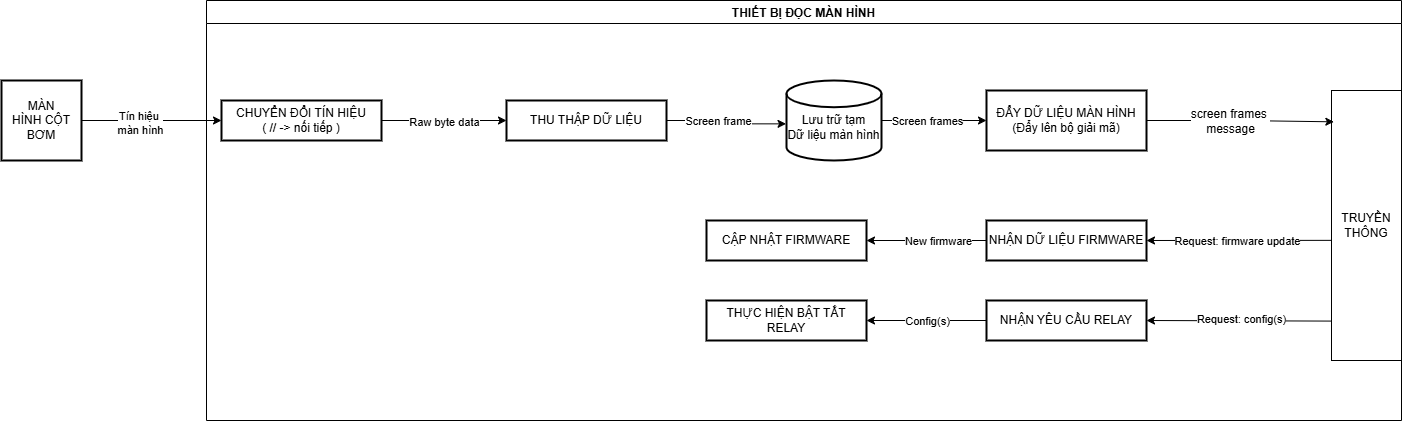
\includegraphics[width=1.0\linewidth]{Figures/Chap3_Device-FunctionBlock.png}
    \caption{Sơ đồ khối chức năng thiết bị đọc ghi màn hình (Device)}
    \label{fig:hinh3.2}
\end{figure}

\textbf{Giải thích các khối chức năng:} 

\begin{itemize}
    \item \textbf{Chuyển đối tín hiệu: }
    \subitem Nếu tín hiệu gửi tới màn hình cột bơm là nối tiếp, khối này đệm tín hiệu nối tiếp tới bộ Thu thập dữ liệu
    \subitem Nếu tín hiệu gửi tới màn hình cột bơm là song song, có nhiều chân dữ liệu, khối này chuyển đổi tín hiệu từ các chân thành tín hiệu nối tiếp -> chuyển đổi thành các SPI frame để đệm tới bộ Thu thập dữ liệu.
    \item \textbf{Thu thập dữ liệu: } Thu thập các byte data tổng hợp thành các screen frame, lưu tạm vào 1 in-mem database.
    \item \textbf{Đẩy dữ liệu lên màn hình: } Thiết bị đọc màn hình tạo 1 message (request message) gồm nhiều screen frame để đẩy lên máy tính local
    \item \textbf{Nhận và cập nhật firmware mới: } Thiết bị đọc màn hình có thể nhận firmware mới từ máy tính local hoặc Logi Service và tự động cập nhật, khởi động lại
    \item \textbf{Nhận và cập nhật relay:} Thiết bị đọc ghi màn hình có thể nhận và thực hiện yêu cầu bật tắt relay 
    \item \textbf{Truyền thông:} Lấy địa chỉ IP, dò tìm địa chỉ của phần mềm giải mã và tự động kết nối. Truyền nhận dữ liệu với phần mềm giải mã thông qua mạng LAN.

\end{itemize}

\subsubsection{Sơ đồ khối chức năng phần mềm giải mã (Device Service)}

\begin{figure}[!ht]
    \centering
    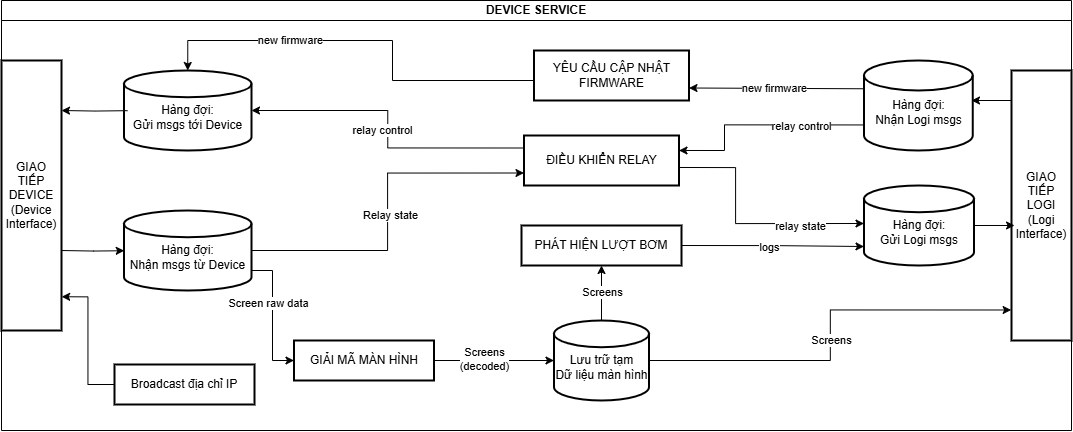
\includegraphics[width=1.0\linewidth]{Figures/Chap3_DeviceService-function-block.png}
    \caption{Sơ đồ khối chức năng phần mềm giải mã và chốt phiên bơm (Device Service)}
    \label{fig:hinh3.3}
\end{figure}

\textbf{Giải thích các khối chức năng:}

\begin{itemize}
    \item \textbf{Giao tiếp với Device (Thiết bị đọc ghi màn hình):} 
    \subitem Khối này được thiết kế chạy trên 1 luồng độc lập, nghe các yêu cầu kết nối từ thiết bị đọc ghi màn hình, kiểm tra và giữ kết nối nếu thiết bị hợp lệ 
    \subitem Truyền nhận gói tin với thiết bị đọc ghi và đẩy dữ liệu tới các khối khác để xử lý logic chính.

    \item \textbf{Giao tiếp với giao diện (GUI App):} Giữ kết nối và truyền nhận dữ liệu với phần mềm giao diện bao gồm:
    \subitem Stream dữ liệu màn hình đã giải mã theo thời gian thực.
    \subitem Gửi các phiên bơm (log) phát hiện được và trạng thái relay.
    \subitem Nhận các yêu cầu từ giao diện: cập nhật firmware, relay.
    \item \textbf{Giải mã màn hình và phát hiện phiên bơm:} Giải mã các gói tin dạng byte theo từng loại màn hình để được dữ liệu màn hình thời gian thực (số tiền, lít, đơn giá). Từ đó phát hiện trạng thái của máy (đang dừng và dừng trong bao nhiêu giây, đang tăng, reset) và phát hiện phiên bơm.
    \item \textbf{Cập nhật firmware:} Nhận file firmware từ giao diện, kiểm tra và thực hiện OTA với thiết bị đọc màn hình 
    \item \textbf{Điều khiển relay:} Chuyển tiếp gói tin yêu cầu bật tắt relay tới thiết bị đọc ghi màn hình
\end{itemize}


\subsection{Thiết kế phần cứng thiết bị đọc màn hình}

\subsubsection{Sơ đồ khối phần cứng thiết bị đọc màn hình}


\begin{figure}[!ht]
    \centering
    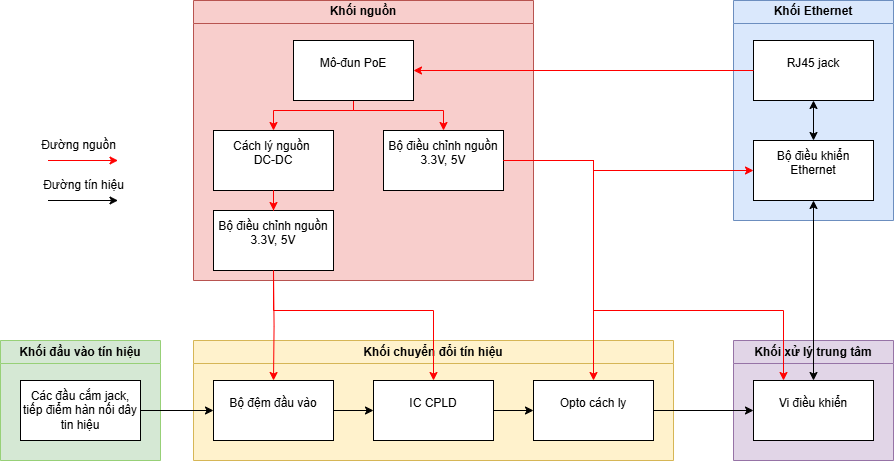
\includegraphics[width=1.0\linewidth]{Figures/Chap3_Device-Hardware-implementation-function-block.png}
    \caption{Sơ đồ khối triển khai phần cứng thiết bị đọc ghi màn hình}
    \label{fig:hinh3.4}
\end{figure}

Thiết bị mạch cứng được cấp nguồn riêng bởi POE Switch. Nguồn và tín hiệu vào được các ly bởi bộ cách ly nguồn DC-DC, các bộ đệm đầu vào và Opto cách ly, đảm bảo không ảnh hưởng tới nguồn cấp của cột bơm cũng như không có tín hiệu hay nhiễu đẩy ngược về cột bơm.

Khối đầu vào tín hiệu và khối chuyển đổi tín hiệu cũng được thiết kế thêm để thu và khảo sát được nhiều loại màn hình khác, phục vụ cho việc mở rộng chức năng hệ thống.

Thiết bị giao tiếp với phần mềm giải mã thông qua mạng LAN, sử dụng khối Ethernet.

\subsubsection{Lựa chọn linh kiện}

\textbf{a.  Khối xử lý trung tâm}

 Yêu cầu lựa chọn:
\begin{itemize}
    \item Có 2 cổng giao tiếp SPI: mục đích để giao tiếp với khối chuyển đổi tín hiệu và với khối Ethernet. 
    \item Bộ nhớ flash lớn hơn 220KB (chứa được 2 firmware, mỗi firm ~ 110kB)
\end{itemize}

Từ những yêu cầu trên , lựa chọn STM32F407VET6 là vi điều khiển xử lý trung tâm. Các tính năng nổi bật của STM32F407VET6:

\begin{itemize}
    \item Vi điều khiển sử dụng lõi ARM Cortex-M4 32-bit, tốc độ tối đa 168 MHz, tích hợp bộ xử lý dấu chấm động (FPU) và tập lệnh DSP, phù hợp cho các ứng dụng điều khiển và xử lý tín hiệu thời gian thực.
    
    \item Bộ nhớ Flash Main Memory 512 KB, được chia thành các sector như sau:  
    
    \begin{itemize}
        \item Sector 0-3: mỗi sector 16 KB  
        \item Sector 4: 64 KB  
        \item Sector 5, 6 và 11: mỗi sector 128-KB  
    \end{itemize}

    \item Cho phép linh hoạt khi lưu nhiều firmware (ví dụ dual-bank firmware upgrade), hoặc phân vùng cho bootloader, data log, cấu hình...

    \item Tích hợp 3 cổng SPI (SPI1, SPI2, SPI3), hỗ trợ chế độ master/slave, tốc độ tối đa đến 42 MHz (SPI1) và 21 MHz (SPI2/SPI3). Phù hợp cho các giao tiếp tốc độ cao như ADC ngoại vi và module Ethernet SPI.

    \item Có tổng cộng 17 bộ Timer, gồm 12 timer 16-bit và 2 timer 32-bit. Hỗ trợ nhiều chế độ: PWM, encoder, input capture, output compare, rất hữu ích trong điều khiển động cơ, đo thời gian hoặc phát xung.

    \item Hỗ trợ nhiều chuẩn giao tiếp ngoại vi: UART, I2C, USB OTG, CAN, SDIO, Ethernet MAC - thuận tiện cho mở rộng và kết nối các module chức năng khác.

    \item Hoạt động với điện áp 1.8 V đến 3.6 V, hỗ trợ các chế độ tiết kiệm năng lượng như Sleep, Stop, và Standby - phù hợp cho ứng dụng nhúng có yêu cầu tiêu thụ điện thấp.
\end{itemize}


\begin{figure}[!ht]
    \centering
    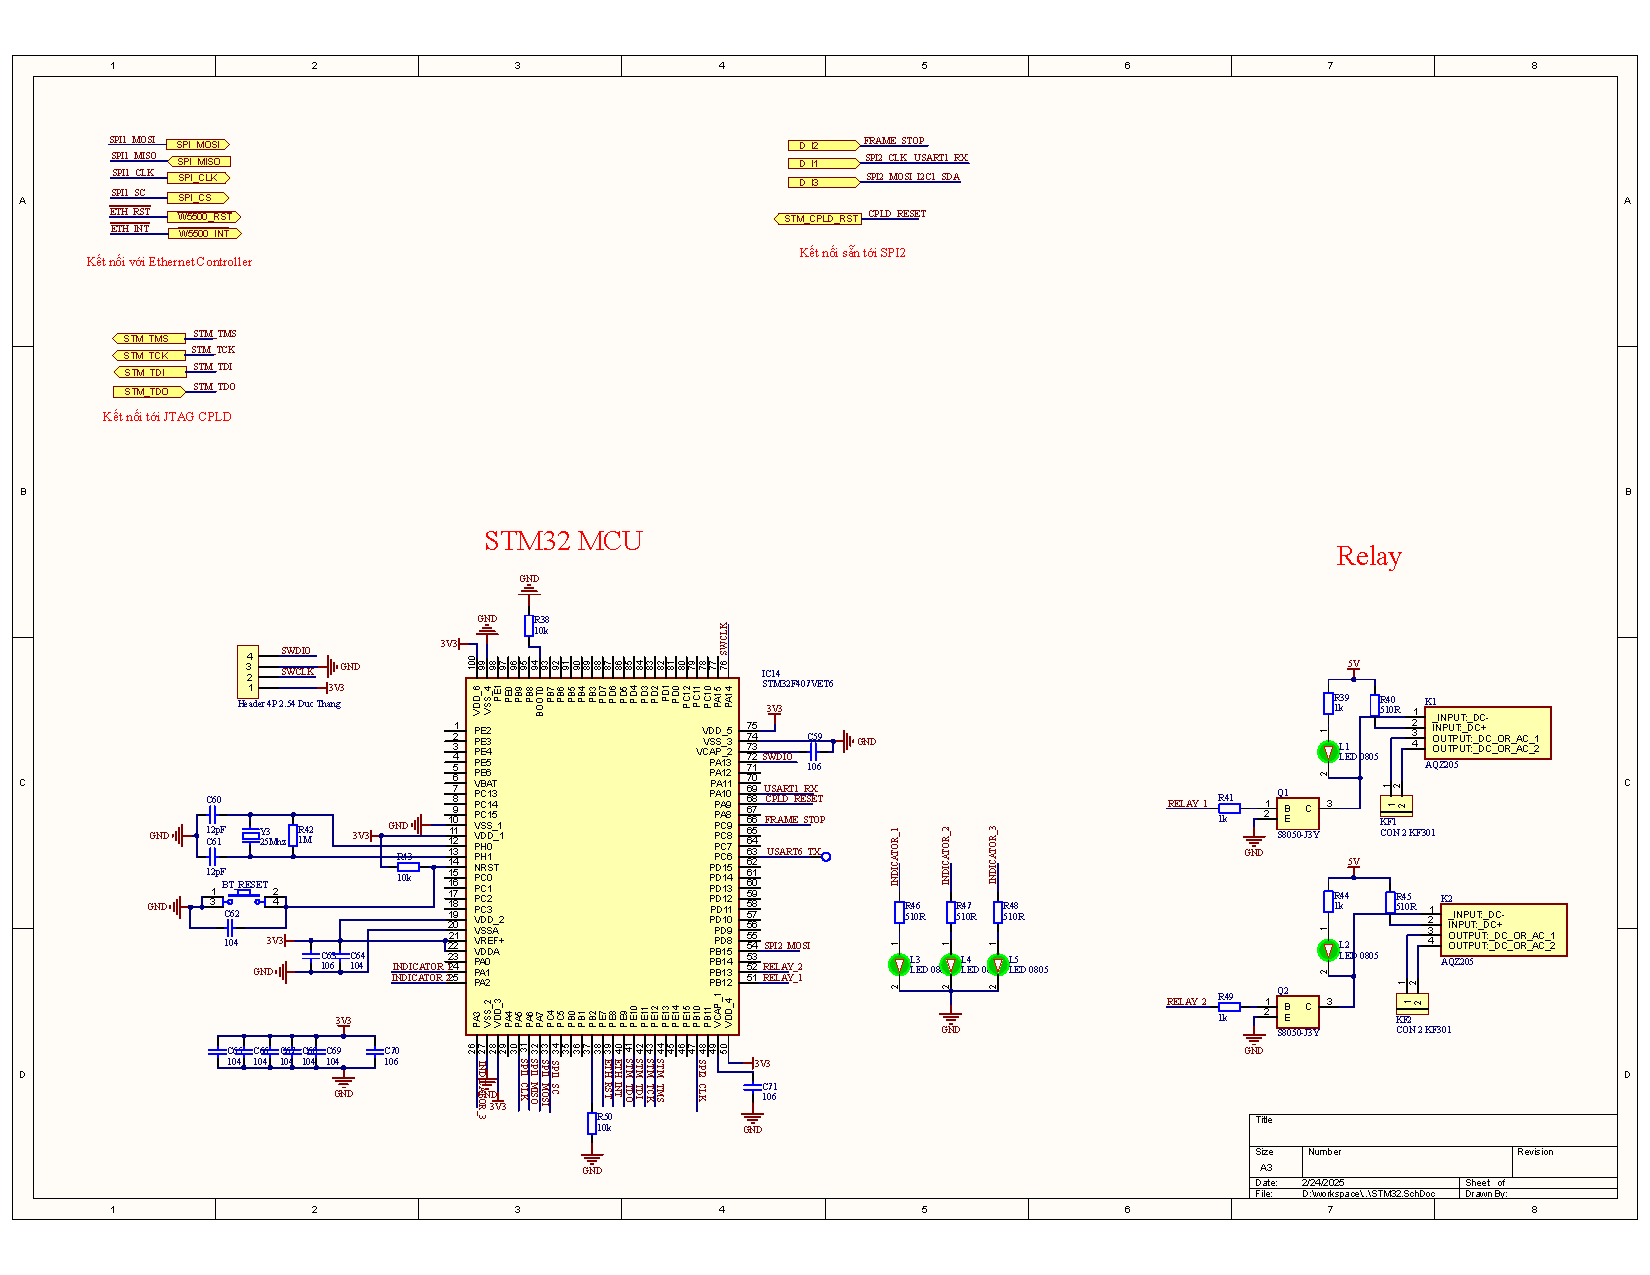
\includegraphics[width=1.0\linewidth]{Figures/Chap3_STM32-principle.pdf}
    \caption{Sơ đồ nguyên lý khối xử lý trung tâm}
    \label{fig:hinh3.5}
\end{figure}


\hspace{0.8cm} Sơ đồ nguyên lý mạch:

\begin{itemize}
    \item Nguồn cấp 3.3V được đưa vào các chân VDD và Vref của module, các chân VSS được nối đất. Thiết kế nguồn nối với đất qua các tụ Bypass có nhiệm vụ lọc nhiễu cao tần cho nguồn nuôi vi điều khiển.
    \item Sử dụng SPI1 để giao tiếp với chip Ethernet. SPI2 để giao tiếp với khối chuyển đổi dữ liệu
    \item Các chân PA1, PA2, PA3 điều khiển đèn báo led 
    \item Reset STM32 được thực hiện khi chân NRST hạ xuống mức 0:
    \begin{itemize}
        \item Điện trở kéo lên 10K$\Omega$
        \item Tụ điện: C = 100nF, giúp tạo xung reset ngắn nhưng đủ để tái khởi STM32
    \end{itemize}
    \item Mạch nạp cho STM32:
    \begin{itemize}
        \item Thiết kế mạch nạp theo chuẩn SWD
        \item Hỗ trợ nạp thông qua mạch nạp STLink
    \end{itemize}

\end{itemize}

\textbf{Khối đầu vào tín hiệu}


 Yêu cầu lựa chọn: 

Ngoài việc thu và giải mã loại màn hình ZCheng, khối đầu vào tín hiệu còn cần hỗ trợ các loại đầu vào cho màn hình khác để thu mẫu dữ liệu, phục vụ cho việc giải mã, mở rộng hệ thống sau này. Các loại đầu vào màn hình đã khảo sát được bao gồm:

\begin{itemize}
    \item Đầu vào SPI (cho màn hình ZCheng, đã giải mã được). Loại cáp: 8P 3.96mm. Số chân tín hiệu: 3
    \item Loại cáp: 5P 3.96mm, số chân tín hiệu: 2
    \item Loại cáp: IDE 10. Số chân tín hiệu 3
    \item Loại cáp: IDE 40. Số chân tín hiệu 30
\end{itemize}

Với danh sách loại đầu vào ở trên, thiết kế khối đầu vào tín hiệu gồm các đầu jack cắm và tiếp điểm hàn để đấu nối dây điên. Khối gồm 2 phần: 

\begin{itemize}
    \item Các đầu cắm cáp: hỗ trợ các loại cáp đã khảo sát.
    \item Các điểm hàn nối dây: Trường hợp các loại màn hình khác, sẽ hàn các đường tín hiệu đó thông qua các đầu tiếp điểm hàn, kèm dây điện nối (nếu cần). Vị trí mối hàn, đấu dây sẽ cố định theo từng loại tín hiệu màn hình.
\end{itemize}

Số chân tối đa cho khối đầu vào tín hiệu là 40 chân.

\begin{figure}[!ht]
    \centering
    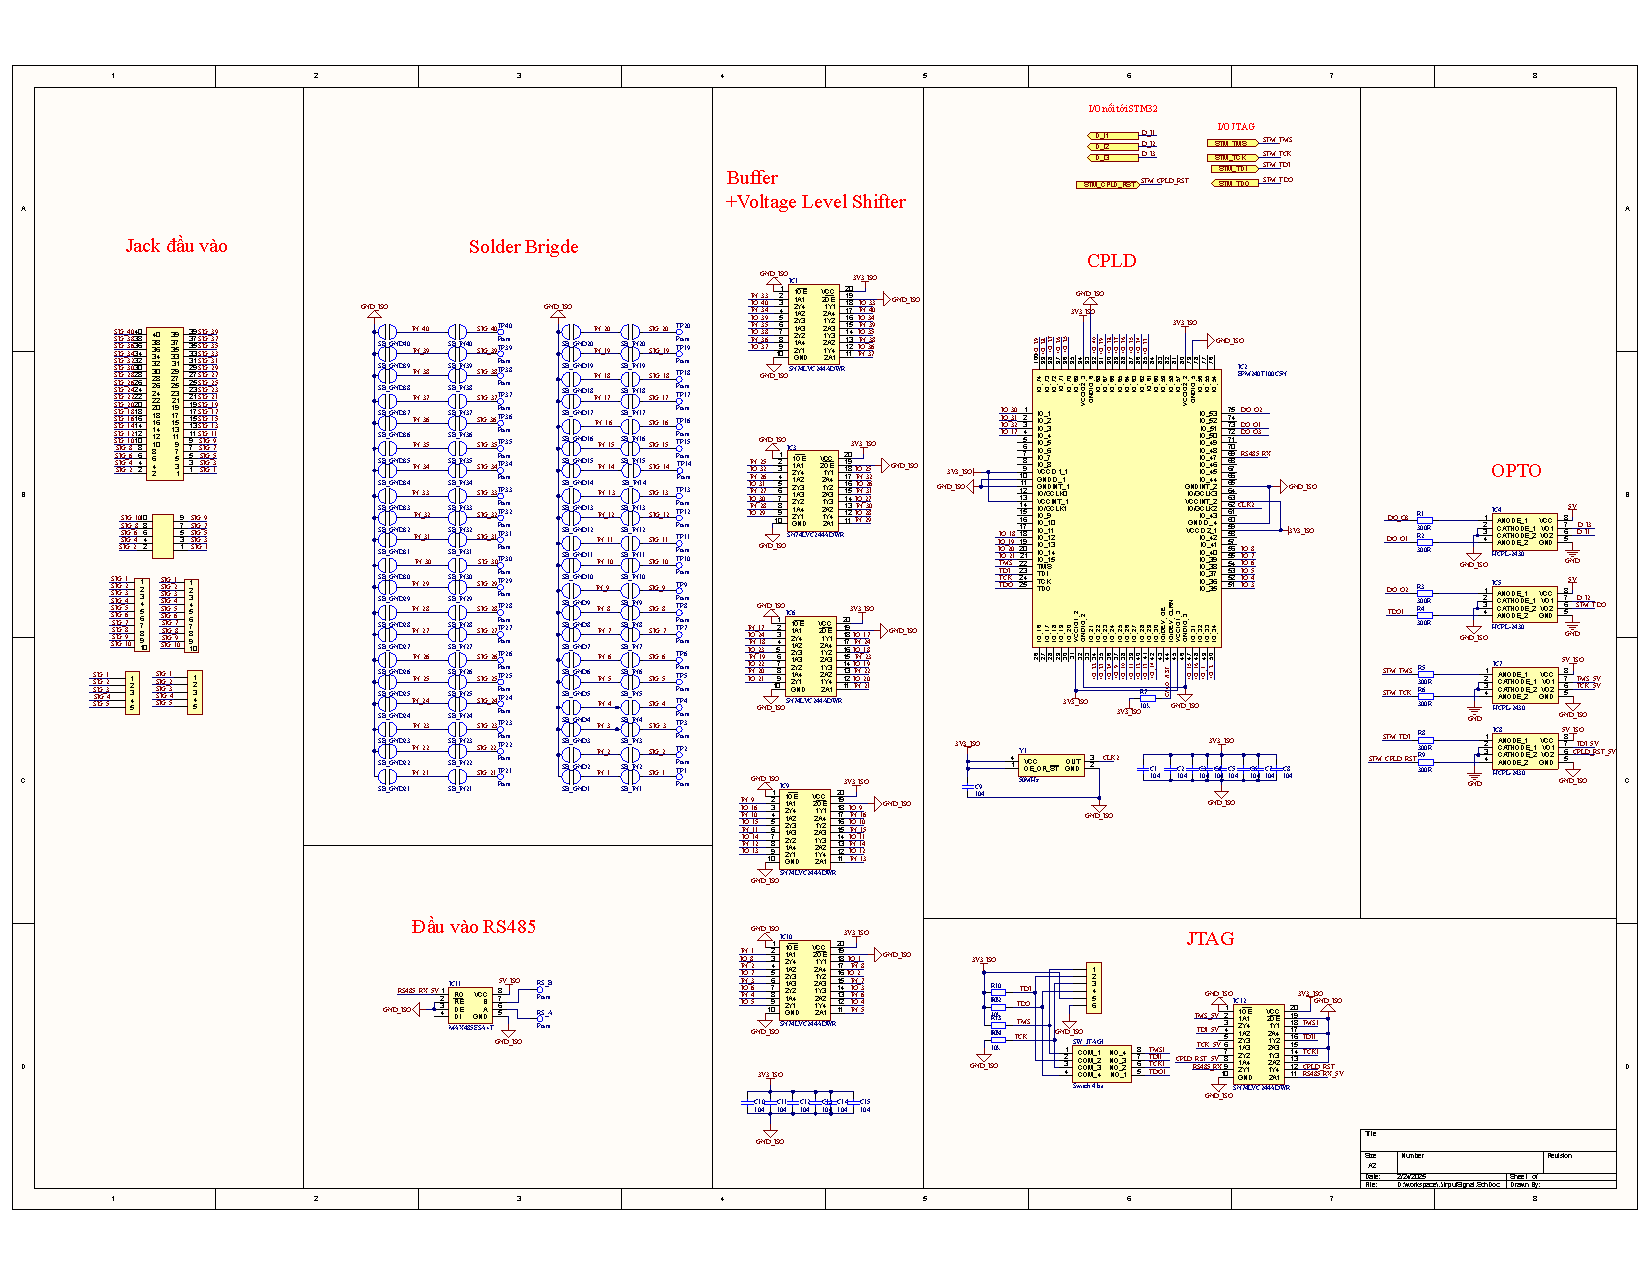
\includegraphics[width=1.0\linewidth]{Figures/Chap3_Input-signal-block-principle.pdf}
    \caption{Sơ đồ nguyên lý khối đầu vào tín hiệu}
    \label{fig:hinh3.6}
\end{figure}
























\newpage
%% --------------------------------------------------%%
%------------ CHAPTER 4 ---------------------------%
%%-----------------------------------------------------%

\section*{CHƯƠNG 4. MÔ PHỎNG VÀ KẾT QUẢ}
    \addcontentsline{toc}{section}{\numberline{} CHƯƠNG 4. MÔ PHỎNG VÀ KẾT QUẢ}
\setcounter{section}{4}
    \setcounter{figure}{0}
        \setcounter{table}{0}
            \setcounter{equation}{0}

%--------------------------------------------------------%

Các kết quả được thể hiện tại đây ...

\newpage


% CONCLUSIONS
\section*{KẾT LUẬN}
    \phantomsection\addcontentsline{toc}{section}{\numberline {}KẾT LUẬN}



\newpage

% REFERENCES
\phantomsection\addcontentsline{toc}{section}{\numberline {}TÀI LIỆU THAM KHẢO}

\bibliography{citation}
\newpage

% APPENDIX
\section*{PHỤ LỤC}
    \phantomsection\addcontentsline{toc}{section}{\numberline{} PHỤ LỤC}

    \setcounter{section}{0}
    \setcounter{subsection}{0}
        \setcounter{figure}{0}
            \setcounter{table}{0}

\appendix

\counterwithin{figure}{section}

% \section{Công trình công bố liên quan}\label{sec:cong_bo}

\section{Một số phương pháp đo và hiệu chuẩn}


Phụ lục cần thêm (nếu có)
...



\end{document}